\documentclass{article}

\usepackage{amsmath}
\usepackage{amssymb}
\usepackage{amsthm}
\usepackage{tikz}
\usepackage{listings}
\usepackage{hyperref}
\usepackage[margin=1in]{geometry}
\usepackage{xcolor}

\usetikzlibrary{arrows.meta, calc, positioning, decorations.pathreplacing}

\definecolor{codebg}{RGB}{245,245,245}
\definecolor{codekw}{RGB}{0,0,180}
\definecolor{codestr}{RGB}{0,128,0}
\definecolor{codecomment}{RGB}{120,120,120}

\lstset{
  language=JavaScript,
  basicstyle=\small\ttfamily,
  backgroundcolor=\color{codebg},
  keywordstyle=\color{codekw},
  stringstyle=\color{codestr},
  commentstyle=\color{codecomment}\itshape,
  showstringspaces=false,
  breaklines=true,
  frame=single,
  numbers=left,
  numberstyle=\tiny\color{gray},
  xleftmargin=2em,
  framexleftmargin=2em,
}

\newtheorem{example}{Example}
\newtheorem{exercise}{Exercise}

\title{Guide 09: Bounding Boxes and Screen Rects}
\author{web-3d-panel-navigation math curriculum}
\date{}

\begin{document}
\maketitle

\section{Why this matters}

When the camera flies into a panel, the page content fades in through a CSS
\texttt{clip-path: inset(...)} window that grows from the panel's projected silhouette
on screen until it covers the whole viewport. To drive that, the project needs two
geometric primitives. First, an \emph{axis-aligned bounding box (AABB)} in world space,
computed once across all panels in
\texttt{calculateAllPlanesBoundingBox} (\texttt{src/projection.ts:23--48}); this is later
used by guide 11's tiling code to frame an overview shot. Second, a
\emph{screen rect} -- four pixel insets from the viewport edges -- computed per panel by
\texttt{getPlaneScreenRect} (\texttt{src/projection.ts:126--152}) and converted to a CSS
clip-path string by \texttt{screenRectToClipPath} (\texttt{src/projection.ts:199--210}).
The screen rect drives the reveal animation, and during transitions
\texttt{lerpScreenRect} (\texttt{src/projection.ts:215--226}) interpolates between
the panel-shaped clip and the full viewport. The renderer applies the clip in
\texttt{ClipController.setClipRect} (\texttt{src/clip-controller.ts:39--43}).

\section{Building intuition}

\subsection{An AABB contains a point set}

An axis-aligned bounding box (AABB) is the smallest axis-aligned rectangle (in 2D) or box
(in 3D) that contains a given set of points. ``Axis-aligned'' means the box's sides are
parallel to the coordinate axes -- never tilted. Below, three rotated quads each have four
corners (eight points total). The dashed rectangle is the unique smallest axis-aligned
rectangle containing all those corners.

\begin{center}
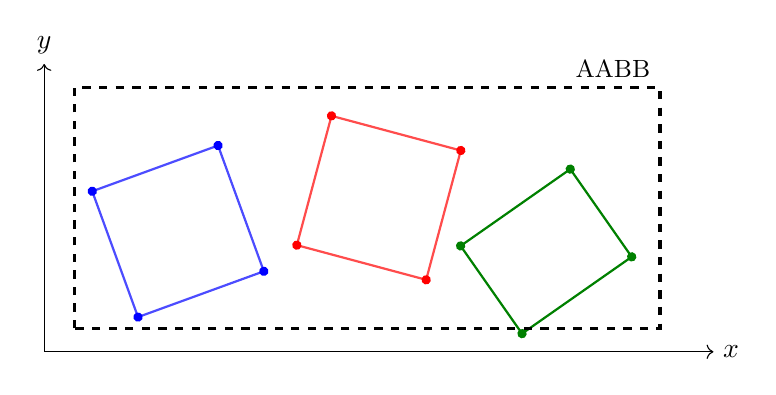
\begin{tikzpicture}[scale=0.85]
  % Three rotated rectangles
  \begin{scope}[rotate around={20:(1.5,1.5)}]
    \draw[blue!70,thick] (0.5,0.5) rectangle (2.5,2.5);
    \fill[blue] (0.5,0.5) circle (2pt);
    \fill[blue] (2.5,0.5) circle (2pt);
    \fill[blue] (2.5,2.5) circle (2pt);
    \fill[blue] (0.5,2.5) circle (2pt);
  \end{scope}
  \begin{scope}[rotate around={-15:(4.5,2)}]
    \draw[red!70,thick] (3.5,1) rectangle (5.5,3);
    \fill[red] (3.5,1) circle (2pt);
    \fill[red] (5.5,1) circle (2pt);
    \fill[red] (5.5,3) circle (2pt);
    \fill[red] (3.5,3) circle (2pt);
  \end{scope}
  \begin{scope}[rotate around={35:(7,1.2)}]
    \draw[green!50!black,thick] (6,0.4) rectangle (8,2);
    \fill[green!50!black] (6,0.4) circle (2pt);
    \fill[green!50!black] (8,0.4) circle (2pt);
    \fill[green!50!black] (8,2) circle (2pt);
    \fill[green!50!black] (6,2) circle (2pt);
  \end{scope}

  % Bounding box (computed roughly to enclose all corner points above)
  \draw[dashed, very thick, black] (-0.05, 0.05) rectangle (8.7, 3.65);
  \node[anchor=south east] at (8.7, 3.65) {\small AABB};

  % Axes
  \draw[->] (-0.5,-0.3) -- (9.5,-0.3) node[right] {$x$};
  \draw[->] (-0.5,-0.3) -- (-0.5,4) node[above] {$y$};
\end{tikzpicture}
\end{center}

The AABB is generally \emph{larger} than the union of the rotated quads -- it has to
fill in the diagonal slack -- but it's cheap to compute (one pass of min/max), cheap to
test, and easy to reason about.

\subsection{A screen rect as four insets}

A \texttt{ScreenRect} in this project is not stored as $(x, y, w, h)$. It is stored as
four pixel \emph{insets}: distances from the top, right, bottom, and left edges of the
viewport. That matches the CSS \texttt{inset()} clip-path syntax exactly, so the
conversion to a clip string is just a unit change.

\begin{center}
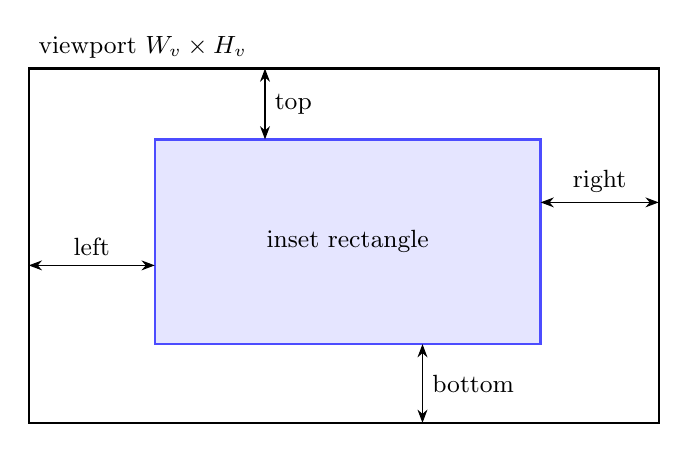
\begin{tikzpicture}[scale=1]
  % Viewport
  \draw[thick] (0,0) rectangle (8,4.5);
  \node[anchor=south west] at (0,4.5) {\small viewport $W_v \times H_v$};

  % Inset rect
  \draw[fill=blue!10, draw=blue!70, thick] (1.6, 1) rectangle (6.5, 3.6);
  \node at (4.05, 2.3) {\small inset rectangle};

  % Top inset arrow
  \draw[<->, >=Stealth] (3, 4.5) -- (3, 3.6);
  \node[right] at (3, 4.05) {\small top};

  % Bottom inset arrow
  \draw[<->, >=Stealth] (5, 0) -- (5, 1);
  \node[right] at (5, 0.5) {\small bottom};

  % Left inset arrow
  \draw[<->, >=Stealth] (0, 2) -- (1.6, 2);
  \node[above] at (0.8, 2) {\small left};

  % Right inset arrow
  \draw[<->, >=Stealth] (6.5, 2.8) -- (8, 2.8);
  \node[above] at (7.25, 2.8) {\small right};
\end{tikzpicture}
\end{center}

\subsection{A rotated panel projects to a non-aligned quad}

When a 3D panel is rotated and projected through the camera, its on-screen silhouette is
generally a \emph{quadrilateral} that is not axis-aligned. The screen-space AABB of the
four projected corners is a tight axis-aligned rectangle around it.

\begin{center}
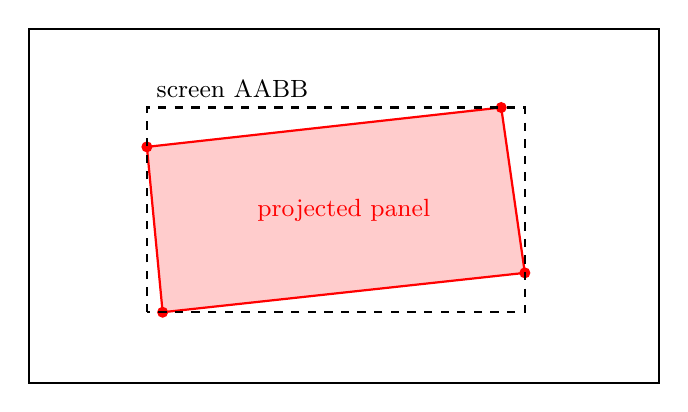
\begin{tikzpicture}[scale=1]
  % Viewport
  \draw[thick] (0,0) rectangle (8,4.5);

  % Projected (non-axis-aligned) quad
  \fill[red!20] (1.7, 0.9) -- (6.3, 1.4) -- (6.0, 3.5) -- (1.5, 3.0) -- cycle;
  \draw[red, thick] (1.7, 0.9) -- (6.3, 1.4) -- (6.0, 3.5) -- (1.5, 3.0) -- cycle;
  \fill[red] (1.7, 0.9) circle (2pt);
  \fill[red] (6.3, 1.4) circle (2pt);
  \fill[red] (6.0, 3.5) circle (2pt);
  \fill[red] (1.5, 3.0) circle (2pt);
  \node[red] at (4, 2.2) {\small projected panel};

  % Screen-space AABB
  \draw[dashed, thick, black] (1.5, 0.9) rectangle (6.3, 3.5);
  \node[anchor=south west] at (1.5, 3.5) {\small screen AABB};
\end{tikzpicture}
\end{center}

The reveal animation grows from the dashed AABB, not from the tilted quad, because CSS
\texttt{inset()} only supports axis-aligned rectangles.

\section{The math}

\subsection{AABB definition}

Let $S \subset \mathbb{R}^3$ be a finite set of points. The axis-aligned bounding box of
$S$ is the Cartesian product
\[
  \mathrm{AABB}(S) = [\min_x, \max_x] \times [\min_y, \max_y] \times [\min_z, \max_z]
\]
where
\[
  \min_x = \min_{\mathbf{p} \in S} p_x,
  \quad \max_x = \max_{\mathbf{p} \in S} p_x,
\]
and analogously for $y$ and $z$. In 2D drop the $z$ component.

This is the smallest box, with sides parallel to the axes, that contains every point of
$S$. ``Smallest'' here is unambiguous: any axis-aligned box containing $S$ must contain
the extreme coordinates, so it must contain $\mathrm{AABB}(S)$.

\paragraph{Why AABBs?}
\begin{itemize}
  \item \textbf{Cheap to compute.} One pass over the points; six min/max updates per
    point. $O(n)$ time, $O(1)$ memory.
  \item \textbf{Cheap to test for overlap.} Two AABBs $A$ and $B$ overlap iff
    $A.\min_x \le B.\max_x$ and $A.\max_x \ge B.\min_x$ on every axis -- six comparisons.
  \item \textbf{Conservative.} The AABB always contains the true region. If the AABB
    misses something, the actual geometry definitely misses it.
\end{itemize}

\subsection{AABB of a union}

If $A$ and $B$ are point sets, then
\[
  \mathrm{AABB}(A \cup B) = \mathrm{AABB}(A) \,\sqcup\, \mathrm{AABB}(B),
\]
where the operation $\sqcup$ on AABBs takes componentwise mins and maxes:
\[
  (A \sqcup B).\min_x = \min(A.\min_x, B.\min_x),
  \quad (A \sqcup B).\max_x = \max(A.\max_x, B.\max_x).
\]
This holds because $\min$ and $\max$ over the union of two sets equal the min/max of the
per-set extremes:
$\min(A \cup B) = \min(\min A, \min B)$.

The operation is commutative ($\min$ and $\max$ are commutative) and associative
($\min$ and $\max$ are associative), so we can fold it over a list of objects in any
order. This is what \texttt{calculateAllPlanesBoundingBox} does: a single accumulator
walks all panels, all corners, and updates a running min/max for each axis.

\subsection{World corners of an oriented panel}

Recall from guide 06 that a panel has a local frame. In its own local space the four
corners sit on a flat rectangle of width $W$ and height $H$ at $z = 0$:
\[
  \mathbf{c}_{\mathrm{local}} \in \left\{
    \big(\pm \tfrac{W}{2},\ \pm \tfrac{H}{2},\ 0\big)
  \right\}.
\]
The local-to-world map applies the panel's rotation and then translates by its position
$\mathbf{c}$. Equivalently, using the basis vectors $\hat{\mathbf{r}}$ (right) and
$\hat{\mathbf{u}}$ (up) of the panel's local frame:
\[
  \mathbf{c}_{\mathrm{world}} = \mathbf{c} + u\,\hat{\mathbf{r}} + v\,\hat{\mathbf{u}},
  \qquad u \in \{-W/2, +W/2\},\ v \in \{-H/2, +H/2\}.
\]
The world AABB of one panel is then
\[
  [\min_x c_{\mathrm{world},x},\ \max_x c_{\mathrm{world},x}] \times \cdots
\]
taken over its four world corners. The world AABB across all panels is, by the union
rule above, the per-axis min/max over all four-corner sets concatenated.

\subsection{Projecting corners to the screen}

Given a world-space corner $\mathbf{p}$, guide 07's pipeline projects it to NDC and then
to pixels:
\begin{align*}
  \mathbf{p}_{\mathrm{NDC}} &= \mathrm{project}(\mathbf{p}, \text{camera}), \\
  x_{\mathrm{px}} &= \tfrac{1}{2}(p_{\mathrm{NDC},x} + 1) \cdot W_v, \\
  y_{\mathrm{px}} &= \tfrac{1}{2}(1 - p_{\mathrm{NDC},y}) \cdot H_v.
\end{align*}
The Y-flip on the second line is because NDC has $+1$ at the top while CSS pixel
coordinates have $0$ at the top.

For an unrotated panel facing the camera straight on, the four projected corners are
already the corners of an axis-aligned rectangle. For a rotated or off-axis panel they
form a general quadrilateral. The screen-space AABB of those four pixel coordinates is
\[
  [x_{\min}, x_{\max}] \times [y_{\min}, y_{\max}],
\]
where each extremum is over the four projected corners.

\subsection{Screen rect insets}

The viewport is a $W_v \times H_v$ rectangle in pixel coordinates, with the origin at
the top-left. The screen rect is the inset of an inner rectangle inside the viewport:
\begin{align*}
  \text{top}    &= \max(0,\ y_{\min}), \\
  \text{right}  &= \max(0,\ W_v - x_{\max}), \\
  \text{bottom} &= \max(0,\ H_v - y_{\max}), \\
  \text{left}   &= \max(0,\ x_{\min}).
\end{align*}
The clamp $\max(0, \cdot)$ handles the case where a projected corner lands outside the
viewport (which gives a negative inset) -- a CSS \texttt{inset()} with a negative value
isn't what we want, so we treat ``outside'' the same as ``flush against the edge.''

Geometrically, the inset rectangle has corners
$(\text{left},\ \text{top})$ and $(W_v - \text{right},\ H_v - \text{bottom})$.

\subsection{CSS clip-path conversion}

CSS clip-path \texttt{inset()} accepts pixels or percentages. The project uses
percentages so the clip survives viewport resizes during a transition. Converting:
\[
  \text{top}\% = \frac{\text{top (px)}}{H_v} \cdot 100,
  \quad \text{right}\% = \frac{\text{right (px)}}{W_v} \cdot 100,
\]
and so on. The resulting CSS string is
\[
  \texttt{inset(top\%\ right\%\ bottom\%\ left\%)}.
\]
That's exactly \texttt{screenRectToClipPath}.

\subsection{Lerping screen rects}

A screen rect lives in $\mathbb{R}^4$ (four insets), so linear interpolation is
componentwise. For a parameter $t \in [0, 1]$ and rects $A$, $B$:
\[
  \mathrm{lerp}(A, B, t).k = A.k + (B.k - A.k) \cdot t,
  \qquad k \in \{\text{top}, \text{right}, \text{bottom}, \text{left}\}.
\]
This is exactly \texttt{lerpScreenRect}. Note that lerping in the inset (pixel) space is
\emph{not} the same as lerping the projected corners in NDC space and then converting
back -- the difference becomes important in guide 12.

\section{In this codebase}

\subsection{The world AABB across all planes}

\begin{lstlisting}
export function calculateAllPlanesBoundingBox(
  configs: ZoomPlaneConfig[],
  scale: number
): BoundingBox {
  if (configs.length === 0) {
    return { minX: 0, maxX: 0, minY: 0, maxY: 0, minZ: 0, maxZ: 0 };
  }

  let minX = Infinity, maxX = -Infinity;
  let minY = Infinity, maxY = -Infinity;
  let minZ = Infinity, maxZ = -Infinity;

  for (const config of configs) {
    const corners = getPlaneWorldCorners(config, scale);
    for (const corner of corners) {
      minX = Math.min(minX, corner.x);
      maxX = Math.max(maxX, corner.x);
      minY = Math.min(minY, corner.y);
      maxY = Math.max(maxY, corner.y);
      minZ = Math.min(minZ, corner.z);
      maxZ = Math.max(maxZ, corner.z);
    }
  }

  return { minX, maxX, minY, maxY, minZ, maxZ };
}
\end{lstlisting}

The mins start at $+\infty$ and the maxes at $-\infty$ -- the identity element of
$\min$ and $\max$ respectively. The double loop is the AABB-of-union rule from
\S 3.2 unrolled: each per-panel AABB is implicitly absorbed into the running totals.
The empty-list early return picks the convention $(0,0,0,0,0,0)$ rather than letting
infinities leak out.

\subsection{World corners of one panel}

This function was the centerpiece of guide 06; here we just remind ourselves where the
input to the AABB comes from.

\begin{lstlisting}
export function getPlaneWorldCorners(
  config: ZoomPlaneConfig,
  scale: number
): THREE.Vector3[] {
  const halfWidth = (config.width * scale) / 2;
  const halfHeight = (config.height * scale) / 2;

  const localCorners = [
    new THREE.Vector3(-halfWidth,  halfHeight, 0),  // top-left
    new THREE.Vector3( halfWidth,  halfHeight, 0),  // top-right
    new THREE.Vector3( halfWidth, -halfHeight, 0),  // bottom-right
    new THREE.Vector3(-halfWidth, -halfHeight, 0),  // bottom-left
  ];

  const euler = new THREE.Euler(...config.rotation);
  const position = new THREE.Vector3(...config.position);

  return localCorners.map(corner => {
    const worldCorner = corner.clone();
    worldCorner.applyEuler(euler);
    worldCorner.add(position);
    return worldCorner;
  });
}
\end{lstlisting}

The four \texttt{localCorners} are the $(\pm W/2, \pm H/2, 0)$ point set. The
\texttt{applyEuler} step rotates them by the panel's Euler triple, and \texttt{add} is
the world translation. After this, each corner is in world coordinates, ready to feed
either an AABB or the screen projection.

\subsection{The screen rect of one panel}

\begin{lstlisting}
export function getPlaneScreenRect(
  config: ZoomPlaneConfig,
  scale: number,
  camera: THREE.Camera,
  viewportWidth: number,
  viewportHeight: number
): ScreenRect {
  const worldCorners = getPlaneWorldCorners(config, scale);
  const screenCorners = worldCorners.map(corner =>
    projectToScreen(corner, camera, viewportWidth, viewportHeight)
  );

  const xs = screenCorners.map(c => c.x);
  const ys = screenCorners.map(c => c.y);

  const minX = Math.min(...xs);
  const maxX = Math.max(...xs);
  const minY = Math.min(...ys);
  const maxY = Math.max(...ys);

  return {
    top: Math.max(0, minY),
    right: Math.max(0, viewportWidth - maxX),
    bottom: Math.max(0, viewportHeight - maxY),
    left: Math.max(0, minX)
  };
}
\end{lstlisting}

The function reads top to bottom as the math reads: get world corners, project each one
to pixels, take the screen-space AABB, then convert that AABB to four insets clamped at
zero. The function it calls -- \texttt{projectToScreen} -- is exactly the
NDC-and-Y-flip mapping from \S 3.4.

\subsection{Pixel insets to a CSS clip-path string}

\begin{lstlisting}
export function screenRectToClipPath(
  rect: ScreenRect,
  viewportWidth: number,
  viewportHeight: number
): string {
  const topPercent = (rect.top / viewportHeight) * 100;
  const rightPercent = (rect.right / viewportWidth) * 100;
  const bottomPercent = (rect.bottom / viewportHeight) * 100;
  const leftPercent = (rect.left / viewportWidth) * 100;

  return `inset(${topPercent.toFixed(2)}% ${rightPercent.toFixed(2)}% ${bottomPercent.toFixed(2)}% ${leftPercent.toFixed(2)}%)`;
}
\end{lstlisting}

The top and bottom insets are normalized by the viewport \emph{height}; the left and
right insets by the viewport \emph{width}. The two-decimal rounding is purely cosmetic;
CSS will accept any precision.

\subsection{Lerping a screen rect}

\begin{lstlisting}
export function lerpScreenRect(
  from: ScreenRect,
  to: ScreenRect,
  t: number
): ScreenRect {
  return {
    top:    from.top    + (to.top    - from.top)    * t,
    right:  from.right  + (to.right  - from.right)  * t,
    bottom: from.bottom + (to.bottom - from.bottom) * t,
    left:   from.left   + (to.left   - from.left)   * t
  };
}
\end{lstlisting}

This is the four-component lerp from \S 3.7. The transition timeline calls this each
frame, then \texttt{ClipController.setClipRect} pipes the result through
\texttt{screenRectToClipPath} into the live CSS.

\section{Worked examples}

\begin{example}[World AABB of two panels]
Two panels:
\begin{itemize}
  \item Panel A: $W = 1600$, $H = 900$, position $(0, 0, -1500)$, rotation $(0, 0, 0)$.
  \item Panel B: $W = 800$, $H = 600$, position $(2000, 100, -1500)$, rotation $(0, 0, 0)$.
\end{itemize}
At \texttt{scale = 1}, find the world AABB containing both.

Panel A corners: $(\pm 800, \pm 450, -1500)$, four points.
Panel B corners: $(2000 \pm 400, 100 \pm 300, -1500) = (1600\text{ or }2400,\ -200\text{ or }400,\ -1500)$.

Per-axis extremes:
\begin{itemize}
  \item $x$: $\min = -800$, $\max = 2400$.
  \item $y$: $\min = -450$, $\max = 450$.
  \item $z$: $\min = -1500$, $\max = -1500$.
\end{itemize}
So the AABB is $[-800, 2400] \times [-450, 450] \times \{-1500\}$.
\end{example}

\begin{example}[Screen rect of a centered, unrotated panel]
Panel: $W = 1600$, $H = 900$, position $(0, 0, -1500)$, rotation $(0, 0, 0)$,
\texttt{scale = 1}. Camera at the origin, FOV $50^\circ$, aspect $1920/1080$.
Viewport $1920 \times 1080$.

The four world corners are $(\pm 800, \pm 450, -1500)$.

The half-height of the view frustum at $z = -1500$ is
$d \tan(\mathrm{fov}/2) = 1500 \cdot \tan(25^\circ) \approx 1500 \cdot 0.4663 \approx 699.5$.
The half-width is that times the aspect ratio:
$699.5 \cdot (1920/1080) \approx 1243.5$.

NDC $x$ of the corner $(800, \cdot, -1500)$ is $800 / 1243.5 \approx 0.6434$. NDC $y$ of
$(\cdot, 450, -1500)$ is $450 / 699.5 \approx 0.6433$.

Convert to pixels (origin top-left, $y$ flipped):
\begin{align*}
  x_{\mathrm{px}} &\in \tfrac{1}{2}(\pm 0.6434 + 1) \cdot 1920
                  \approx \{343.3,\ 1576.7\}, \\
  y_{\mathrm{px}} &\in \tfrac{1}{2}(1 \mp 0.6433) \cdot 1080
                  \approx \{192.6,\ 887.4\}.
\end{align*}
Screen-space AABB: $[343.3,\ 1576.7] \times [192.6,\ 887.4]$.

Insets:
\begin{align*}
  \text{top}    &= \max(0,\ 192.6) = 192.6, \\
  \text{right}  &= \max(0,\ 1920 - 1576.7) = 343.3, \\
  \text{bottom} &= \max(0,\ 1080 - 887.4) = 192.6, \\
  \text{left}   &= \max(0,\ 343.3) = 343.3.
\end{align*}
The result is symmetric, as expected for a centered, unrotated panel.
\end{example}

\begin{example}[Lerping toward full reveal]
Start with the screen rect from the previous example,
$A = (192.6,\ 343.3,\ 192.6,\ 343.3)$, and lerp toward
$B = (0,\ 0,\ 0,\ 0)$ -- the full viewport -- at $t = 0.4$.

Componentwise: $\mathrm{top} = 192.6 + (0 - 192.6) \cdot 0.4 = 115.56$.
By the same arithmetic on each component,
$\mathrm{lerp}(A, B, 0.4) = (115.56,\ 205.98,\ 115.56,\ 205.98)$.

Converted to a clip-path against a $1920 \times 1080$ viewport:
top $= 115.56 / 1080 \approx 10.70\%$, right $= 205.98 / 1920 \approx 10.73\%$, etc.
The CSS string is approximately \texttt{inset(10.70\% 10.73\% 10.70\% 10.73\%)}.
\end{example}

\section{Exercises}

\begin{exercise}
Given the point set
$S = \{(1, 2, 3),\ (4, -1, 0),\ (-2, 5, 7),\ (3, 0, -1)\}$,
compute its AABB.
\end{exercise}

\begin{exercise}
A panel has $W = 1000$, $H = 500$, position $(100, 200, -800)$, rotation $(0, 0, 0)$,
\texttt{scale = 1}. Compute its four world corners and its world AABB.
\end{exercise}

\begin{exercise}
For the panel of the previous exercise, the viewport is $1280 \times 720$, the camera is
at the origin with FOV $60^\circ$ and aspect $1280/720$. Compute the screen rect of the
panel.
\end{exercise}

\begin{exercise}
Given a screen rect $A = (50, 100, 50, 100)$ pixels and viewport $1000 \times 500$,
compute the CSS \texttt{inset(...)} string from \texttt{screenRectToClipPath} (use two
decimal places).
\end{exercise}

\begin{exercise}
Given $A = (200, 300, 200, 300)$ and $B = (0, 0, 0, 0)$, compute
$\mathrm{lerp}(A, B, 0.25)$ and $\mathrm{lerp}(A, B, 0.75)$.
\end{exercise}

\subsection*{Conceptual challenge}

\begin{exercise}
Why does \texttt{getPlaneScreenRect} project all four corners and then take the
screen-space AABB, instead of projecting just the panel's center and computing the
on-screen size from the panel's width and height? Give a concrete configuration where
the two approaches disagree.
\end{exercise}

\subsection*{Project-applied challenge}

\begin{exercise}
The project lerps the screen rect during zoom -- four pixel insets, in screen pixels.
Suppose instead it lerped in NDC space: the four projected corners interpolate from
their start positions to the four NDC corners $(\pm 1, \pm 1)$, and the screen rect is
recomputed each frame. Describe one visible difference between the two approaches.
\emph{Hint:} think about what happens when a panel's projected silhouette is far from
square.
\end{exercise}

\section{Where to next}

\begin{itemize}
  \item Guide 10 (slerp): linear interpolation isn't enough for rotations -- the
    transition timeline that calls \texttt{lerpScreenRect} each frame also slerps the
    camera's quaternion.
  \item Guide 11 (the hinge tiling capstone): uses
    \texttt{calculateAllPlanesBoundingBox} to frame an overview shot that fits every
    panel on screen at once.
  \item Guide 12 (adaptive transitions): the formal study of how
    \texttt{lerpScreenRect} feeds into the zoom-in/zoom-out animation, and why the
    interpolation happens in inset space rather than NDC space.
\end{itemize}

\section{Appendix: Solutions}

\subsection*{Exercise 1}
Per-axis extremes: $x \in [-2, 4]$, $y \in [-1, 5]$, $z \in [-1, 7]$. AABB is
$[-2, 4] \times [-1, 5] \times [-1, 7]$.

\subsection*{Exercise 2}
Local corners: $(\pm 500, \pm 250, 0)$. Translate by $(100, 200, -800)$ (no rotation):
\[
  \{(600, 450, -800),\ (-400, 450, -800),\ (600, -50, -800),\ (-400, -50, -800)\}.
\]
World AABB: $[-400, 600] \times [-50, 450] \times \{-800\}$.

\subsection*{Exercise 3}
At distance $800$ with $\mathrm{fov} = 60^\circ$:
half-height $= 800 \cdot \tan(30^\circ) \approx 800 \cdot 0.5774 \approx 461.9$;
half-width $= 461.9 \cdot (1280/720) \approx 821.2$.

NDC of $(600, 450, -800)$: $x = 600 / 821.2 \approx 0.7307$,
$y = 450 / 461.9 \approx 0.9742$.
NDC of $(-400, -50, -800)$: $x = -400 / 821.2 \approx -0.4871$,
$y = -50 / 461.9 \approx -0.1083$.

Project the extreme NDC values to pixels. NDC $x$ ranges from $-0.4871$ to $0.7307$, so
\[
  x_{\mathrm{px}} \in [\tfrac{1}{2}(1 - 0.4871) \cdot 1280,\ \tfrac{1}{2}(1 + 0.7307) \cdot 1280]
              \approx [328.3,\ 1107.7].
\]
NDC $y$ ranges from $-0.1083$ to $0.9742$, so (with the Y-flip)
\[
  y_{\mathrm{px}} \in [\tfrac{1}{2}(1 - 0.9742) \cdot 720,\ \tfrac{1}{2}(1 + 0.1083) \cdot 720]
              \approx [9.3,\ 399.0].
\]
Insets:
\begin{align*}
  \text{top}    &\approx 9.3, \\
  \text{right}  &\approx 1280 - 1107.7 = 172.3, \\
  \text{bottom} &\approx 720 - 399.0 = 321.0, \\
  \text{left}   &\approx 328.3.
\end{align*}
The asymmetry (top vs.\ bottom, left vs.\ right) reflects the panel's offset from the
camera's view axis; that's the whole point of doing this with min/max instead of
assuming centered.

\subsection*{Exercise 4}
top $= 50/500 \cdot 100 = 10\%$; right $= 100/1000 \cdot 100 = 10\%$;
bottom $= 50/500 \cdot 100 = 10\%$; left $= 100/1000 \cdot 100 = 10\%$.
The string is \texttt{inset(10.00\% 10.00\% 10.00\% 10.00\%)}.

\subsection*{Exercise 5}
$\mathrm{lerp}(A, B, 0.25) = (150,\ 225,\ 150,\ 225)$;
$\mathrm{lerp}(A, B, 0.75) = (50,\ 75,\ 50,\ 75)$.

\subsection*{Conceptual challenge}
The center-only approach assumes the panel's projected silhouette is centered on its
projected center and has the same on-screen size as a frontal panel of the same
dimensions. That's true \emph{only} when the panel faces the camera straight-on and
sits on the camera's view axis. Counterexample: a panel rotated $30^\circ$ around its
$Y$ axis. Its projected silhouette is foreshortened, no longer centered on the
projected center (perspective makes the near edge larger than the far edge), and
generally not even rectangular. Projecting all four corners and AABBing them in screen
space handles all of this correctly: it gives a tight axis-aligned screen rect around
the actual silhouette.

\subsection*{Project-applied challenge}
Lerping in NDC space means you're interpolating the projected \emph{quad's corners}, not
the screen AABB's edges. After re-AABBing each frame, the screen rect's growth rate
along each edge depends on which corner is currently extreme. For a panel whose
projected silhouette is wider than tall, the NDC lerp would still hit the viewport
edges first along the wider axis, but the inset-lerp grows all four edges at the same
parametric rate. Visually, the inset-space lerp produces a smooth, symmetric reveal
where the four edges each travel their own pixel distance at the same parametric speed;
the NDC-space lerp produces an asymmetric reveal where the wider axis ``finishes'' first
and the narrower axis catches up later. The current implementation chooses the cleaner,
symmetric look.

\end{document}
